\documentclass[12pt]{article}
% Эта строка — комментарий, она не будет показана в выходном файле
\usepackage{ucs}
\usepackage[warn]{mathtext} 
\usepackage[utf8x]{inputenc} % Включаем поддержку UTF8
\usepackage[russian]{babel}  % Включаем пакет для поддержки русского языка
\usepackage{amsmath}
\usepackage{mathtools}
\usepackage{amssymb}
% \usepackage[dvips]{graphicx}
% \graphicspath{{noiseimages/}}
\usepackage[pdftex]{graphicx}

\hoffset=0mm
\voffset=0mm
\textwidth=180mm        % ширина текста
\oddsidemargin=-6.5mm   % левое поле 25.4 - 5.4 = 20 мм
\textheight=240mm       % высота текста 297 (A4) - 40
\topmargin=-15.4mm      % верхнее поле (10мм)
\headheight=5mm      % место для колонтитула
\headsep=5mm          % отступ после колонтитула
\footskip=8mm         % отступ до нижнего колонтитула


\begin{document}
    \author {Жарков Андрей 496}
    \title {Лабораторная работа 1.2 \\ Определение моментов инерции твердых тел с помощью трифилярного подвеса}
    \maketitle{}   
    
    \indent
    \textbf{Цель работы:} измерение момента инерции ряда тел и сравнение результатов с расчетами по теоретическим формулам; проверка аддттивности моментов инерции и справедливости формулы Гюйгенса– Штейнера.
    \\\newline
    \indent
    \textbf{В работе используются:} трифилярный подвес, секундомер, счетчик числа колебаний, набор тел, момент инерции которых надлежит измерить (диск, стержень, полый цилиндр и другие).
    \\\newline
    
    \textbf{Определение.} Моментом инерции твердого тела (или системы тел) относительно выбранной оси, называется величина, определяемая соотношением: 
    \begin{equation}
              I = \int r^2dm
    \end{equation} 
    
    Из определения момента инерции и по 2-му закону Ньютона для движения материальной точки под действием силы $\vec{F}$, учитывая $v = \omega r$ , уравнение вращательного движения принимает вид:

    \begin{equation}
              I \frac{d\omega}{dt} = M \quad \text{где $M$ - момент силы $\vec{F}$}
    \end{equation} 

    \textbf{Теорема Гюйгенса–Штейнера.} Момент инерции $I$ относительно произвольной оси равен сумме момента инерции $I_0$ относительно оси, параллельной ей и проходящей через центр масс тела, и произведения массы тела $m$ на квадрат расстояния между осями $a_0$:
    \begin{equation}
        I = I_0 + ma^2_0
    \end{equation} \\\newline

    \textbf{Экспериментальная установка.} Будем использовать устройство, показанное на рис. 1 и называемое трифилярным подвесом. Оно состоит из укрепленной на некоторой высоте неподвижной платформы $P$ и подвешенной к ней на трех симметрично расположенных нитях $AA'$, $BB'$ и $CC'$ вращающейся платформы $P'$.

    Платформа $P$ укреплена на кронштейне и снабжена рычагом (на рисунке не показан), при помощи которого в системе создадим крутильные колебания путем небольшого поворота верхней платформы.

    Для счета числа колебаний используется счетчик, состоящий из осветителя (2), фотоэлемента (3) и пересчетного устройства (1). Легкий лепесток, укрепленный на платформе, при колебаниях пересекает световой луч дважды за период. Соответствующие сигналы от фотоэлемента поступают на пересчетное устройство.

    \begin{center} 
        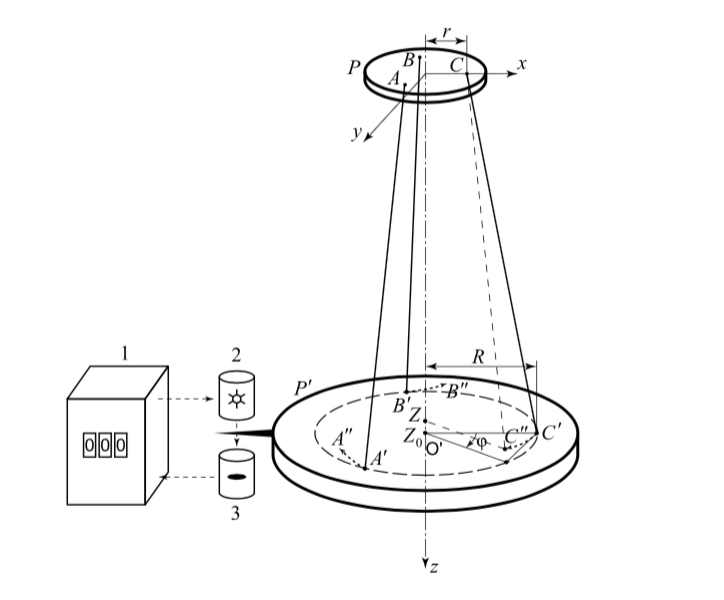
\includegraphics[width=5in]{lab2_1.png} \\ Рис. 1: трифилярный подвес
    \end{center}
    
    \textbf{Уравнение гармонических колебаний.} Уравнение малых колебаний трифилярного подвеса выглядит следующим образом:
    \begin{equation}
        I\ddot{\varphi} + mg \frac{Rr}{z_0}\varphi = 0
    \end{equation} 
    где $I$ — момент инерции тела вместе с платформой, $m$ — их суммарная масса, $z_0$ — расстояние от центра нижней платформы $O'$ до центра верхней $O$ в положении равновесия, а $R$ и $r$ — расстояния от оси вращения до точки крепления нити на нижней и на верхней платформах соответственно (см. рис. 2).

    Решение уравнения (4) представляет собой гармонические колебания:
    \begin{equation}
        \varphi(t) = \varphi_m \sin(2\pi t/T + \theta)
    \end{equation} 
    где амплитуда $\varphi_m$ и фаза $\theta$ определяются начальными условиями, а
    \begin{equation}
        T = 2 \pi \sqrt{\frac{I z_0}{mgRr}}
    \end{equation} 
    положим $k = \frac{gRr}{4\pi^2z_0}$ , эта величина постоянна для данной установки. Тогда момент инерции можно выразить следующим образом:
    \begin{equation}
        I = kmT^2
    \end{equation}

    Таким образом, полученные формулы позволяют определить момент
    инерции платформы с телом и отдельно платформы по соответствующим периодам крутильных колебаний.

    \textbf{Аддитивность моментов инерции.} Момент инерции самого тела можно вычислить, воспользовавшись аддитивностью $I_{A+B}$ — момент инерции составного тела (A+B) равен сумме моментов инерции его частей A и B :
        \begin{equation}
            I_{A+B} = I_A + I_B
        \end{equation}
        
        
        
       
    
    \textbf{\large Выполнение работы}
    \begin{enumerate} 
        \item \textbf{Параметры установки} \\\newline
            $R = 114.6 \pm 0.5$ мм. \\ $r = 30.5 \pm 0.3$ мм.\\
            $m = 353.4 \pm 0.3$ г. \\ $z_0 = 215 \pm 1$ см.\\ \\
            $\sigma_k = k \sqrt{\varepsilon_R^2 + \varepsilon_r^2 + \varepsilon_{z_0}^2}$ \\
            $ k = (4.04 \pm 0.05)* 10 ^ {-4} м^2/c^2$ \\ \\
            $I_0^{теор} = \frac{m R^2}{2} = (2.32 \pm 0.01) * 10 ^{-3} м^2 * кг$

       \item \textbf{Погрешность измерения периода} \\\newline
	       \begin{table}[ht]
	       	\caption{измерения вермени 10 периодов пустой платформы}
	       	\begin{center}
	       		\begin{tabular}{|c|c|c|c|c|c|c|}
	       			\hline 
	       			$i$ & 1 & 2 & 3 & 4 & 5 & 6 \\
	       			\hline
	       			$t_i$,c & 40.855 & 40.980 & 42.113 & 40.600 & 42.004 & 42.348 \\
	       			\hline
	       		\end{tabular}
	       	\end{center}
	       \end{table}
	       
	       $\sigma_{отд} = \sqrt{\frac{\Sigma (t_i - t_{cp})^2 }{n-1}} \approx 0.3957$ \\
	       $T_{ср} = 4.14 \pm 0.02$ с \\
	       Подберём количество периодов, при котором $\varepsilon$ < 0.005 \\
	       $ N=\frac{ \sigma }{ \varepsilon T_{ср}} = 10 $ \\ \\ \\ \\ \\ \\
	       \\ \\
	       
	   \item \textbf{Проверка аддитивности моментов инерции} \\\newline 
		   \begin{enumerate}
		   	\item \textbf{Кольцо} \\\newline
		   	T = 4.12 $\pm$ 0.02 c \\
		   	m = 731.3 г \\
		   	d = 16,7 см \\
		   	$I_{\text{кольца}}=k(m+m_0)T^2-I_0=5.31 \pm$ 0.07 $м^2$*г \\
		   	$I_{\text{теор}}=\frac{md^2}{4} = 5.23 \pm 0.5$ $м^2$*г \\
		   	
		   	
		   	\item \textbf{Диск} \\\newline
		   	T = 3.44 $\pm$ 0.02 c \\
		   	m = 583.8 г \\
		   	d = 17.2 см \\
		   	$I_{диска}=k(m+m_0)T^2-I_0=2.25 \pm 0.04 $ $м^2$*г \\
		   	$I_{теор}=\frac{md^2}{8} = 2.16 \pm 0.02 $ $м^2$*г \\
		   	
		   	\item \textbf{Кольцо+Диск} \\\newline
		   	T = 3.86 $\pm$ 0.02 c \\
		   	$I_{сумм}=k(m_к+m_д+m_0)T^2-I_0=7.6 \pm 0.1 $ $м^2$*г \\
		   	\text{В пределах погрешности аддитивность моментов инерции выполняется.} \\
		   	
		   	\item \textbf{Брусок} \\\newline
		   	T = 3.43 $\pm$ 0.02 c \\
		   	m = 1191.9 г \\
		   	2.6 * 2.6 * 21.1 см \\
		   	$I_{бруска}=k(m+m_0)T^2-I_0=4.63 \pm 0.07 $ $м^2$*г \\
		   	$I_{теор}=\frac{m}{12}(a^2+b^2) = 4.49 \pm 0.09 $ $м^2$*г \\
		   \end{enumerate}
		   
		   В пределах погрешности эксперементальный и теоретический моменты инерции у тел совпали. \\
		   
		   \pagebreak
		   
	   \item \textbf{Проверка теоремы Гюйгенса-Штейнера} \\\newline
	      $m=764.0г$ \\
	      $d=9.1cм$ \\
	      Расположив диск так, как показано на рис. 2 будем увеличивать h. \\
	      
	      \begin{center} 
	      	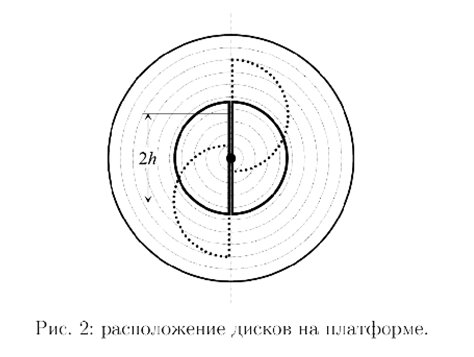
\includegraphics[width=2in]{lab2_2.png}
	      	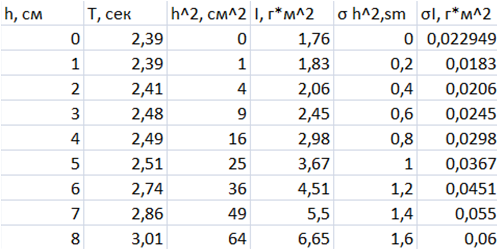
\includegraphics[width=3in]{lab2_table.png} 
	      	\\
	      	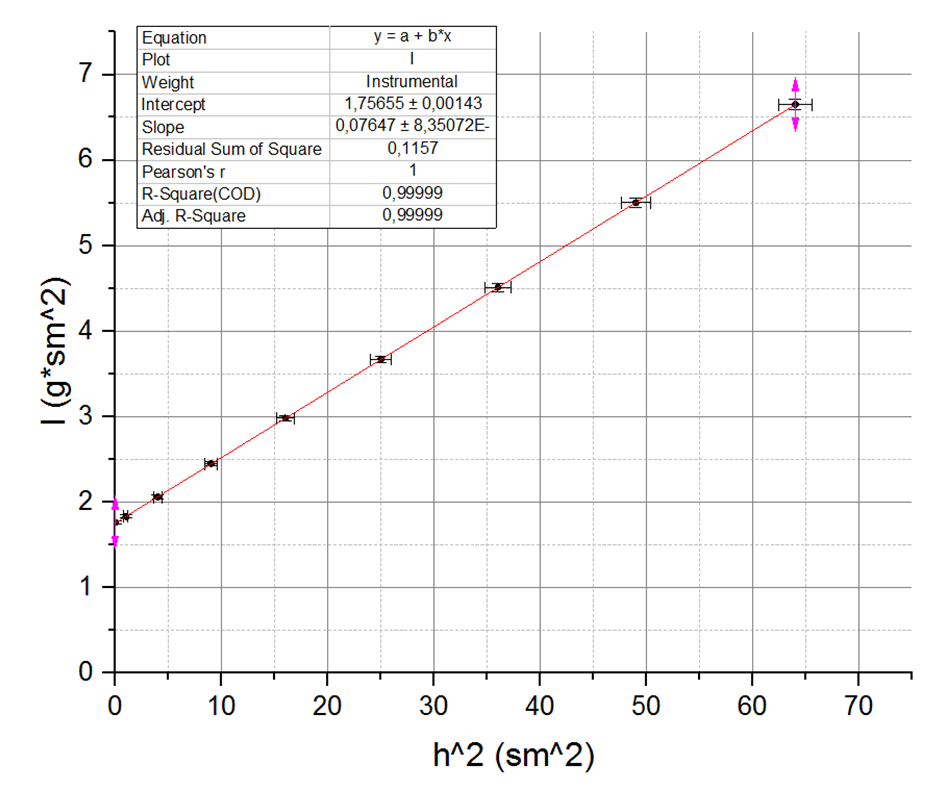
\includegraphics[width=6in]{lab2_plot.png}
	      \end{center}
	      
	      Найденные на графике $I_0 = 1.7565 \pm 0.0014$ г*$м^2$ и коэффициент наклона $m=0.7647 \pm 0.0008$кг. \\
	      $I_{теор}=\frac{md^2}{8} = 1.75 \pm 0.01$ г*$м^2$ \\
	      Как видим, с учётом погрешности, m и $I_0$ совпадают с теоретическими значениями.
	       
		   
		   
	       


    \end{enumerate}     
\end{document}